\subsection{FaBoのピンの種類とケーブルの種類}
FaBoのシールドにはブリックとRaspberry Piを\ruby{繋}{つな}ぐためのピンがあります。ピンの種類には「GPIO」、「A」、「I2C」があります。下の表のように使い方が分けられているので、間違えないように気をつけましょう。\\
\begin{figure}[H]
  \begin{center}
    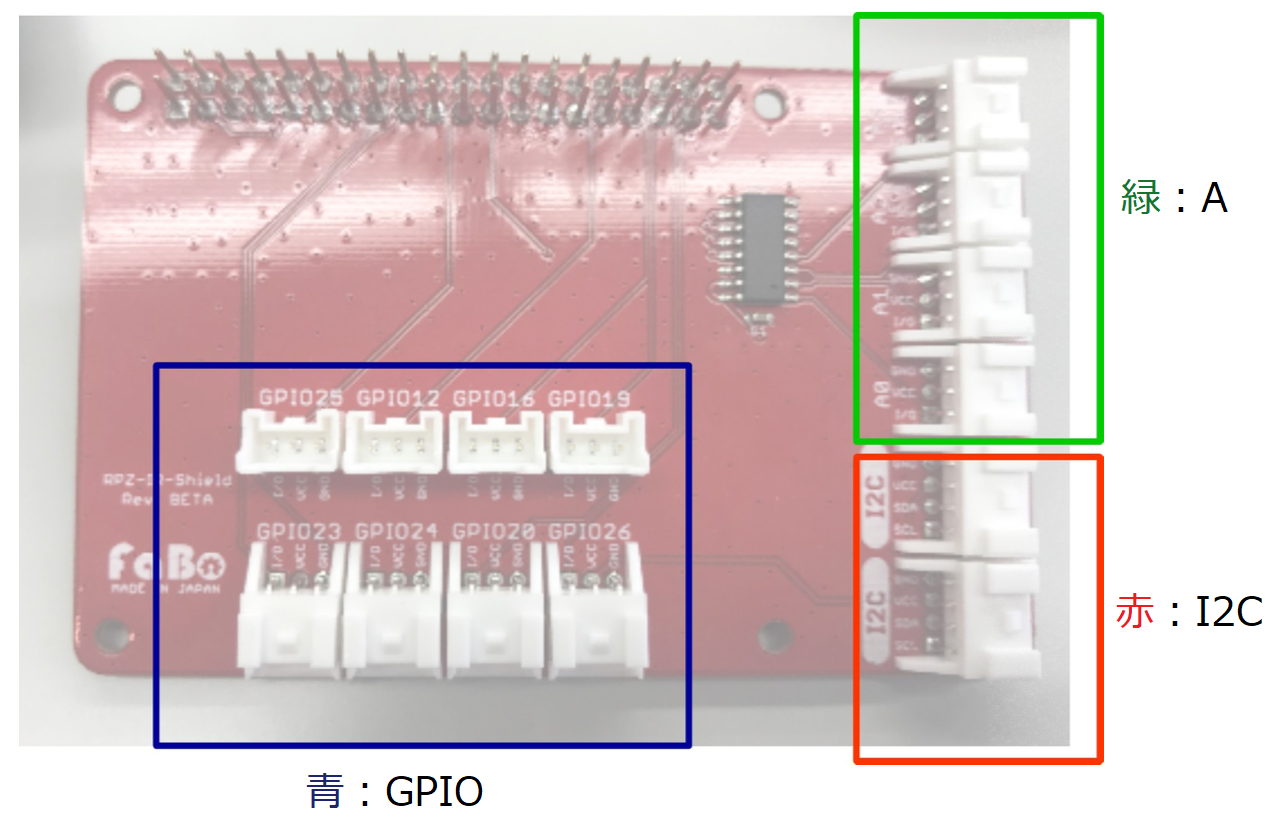
\includegraphics[scale=0.6]{images/chap05/text05-img012.png}
    \caption{Faboシールドのピン配置}
  \end{center}
\end{figure}
\begin{table}[H]
 \centering
 \begin{tabular}{|c|l|} \hline
  GPIO 12 & \multirow{8}{*}{ボタンやスイッチなどのデジタル用のピン} \\ \cline{1-1}
  GPIO 16 & \\ \cline{1-1} GPIO 19 & \\ \cline{1-1} GPIO 20 & \\ \cline{1-1} GPIO 23 & \\ \cline{1-1}
  GPIO 24 & \\ \cline{1-1} GPIO 25 & \\ \cline{1-1} GPIO 26 & \\ \hline
  A0 & \multirow{4}{*}{ボリュームや距離センサーなどのアナログ用のピン} \\ \cline{1-1}
  A1 & \\ \cline{1-1} A2 & \\ \cline{1-1} A3 & \\ \hline
  I2C & \ruby{有機}{ゆう|き}ELディスプレイのような特別な通信のためのピン \\ \hline
 \end{tabular}
\end{table}
今まで使ってきたセンサーボードでは、LEDのピンの割り当てがGPIO17、GPIO18、GPIO22、GPIO24となっており、あらかじめ決められた番号に割り当てられていました。しかしFaBoのGPIOはどの番号につなげても使えます。ただし、プログラムも番号に合わせて書く必要があります。\\
ケーブルは3ピンと4ピンの2種類があります。今回4ピンはゆうきELディスプレイで使います。\\
\begin{figure}[h]
  \begin{center}
    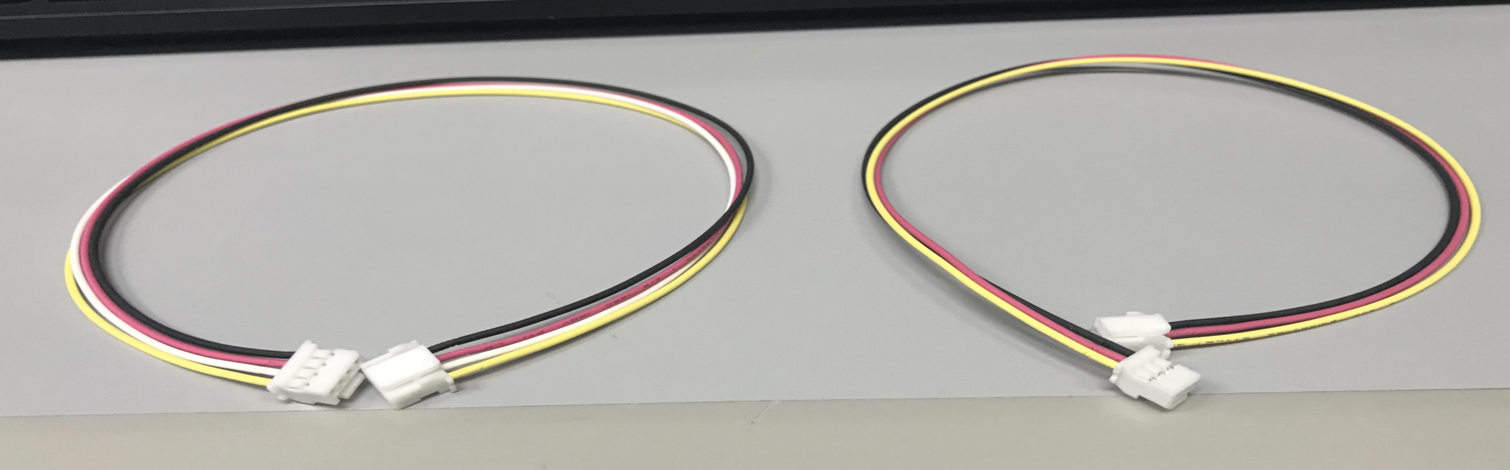
\includegraphics[scale=0.6]{images/chap05/text05-img013.png}
    \caption{4ピンケーブルと3ピンケーブル(全体)}
  \end{center}
\end{figure}
\begin{figure}[H]
  \begin{minipage}[t]{0.48\columnwidth}
    \centering
    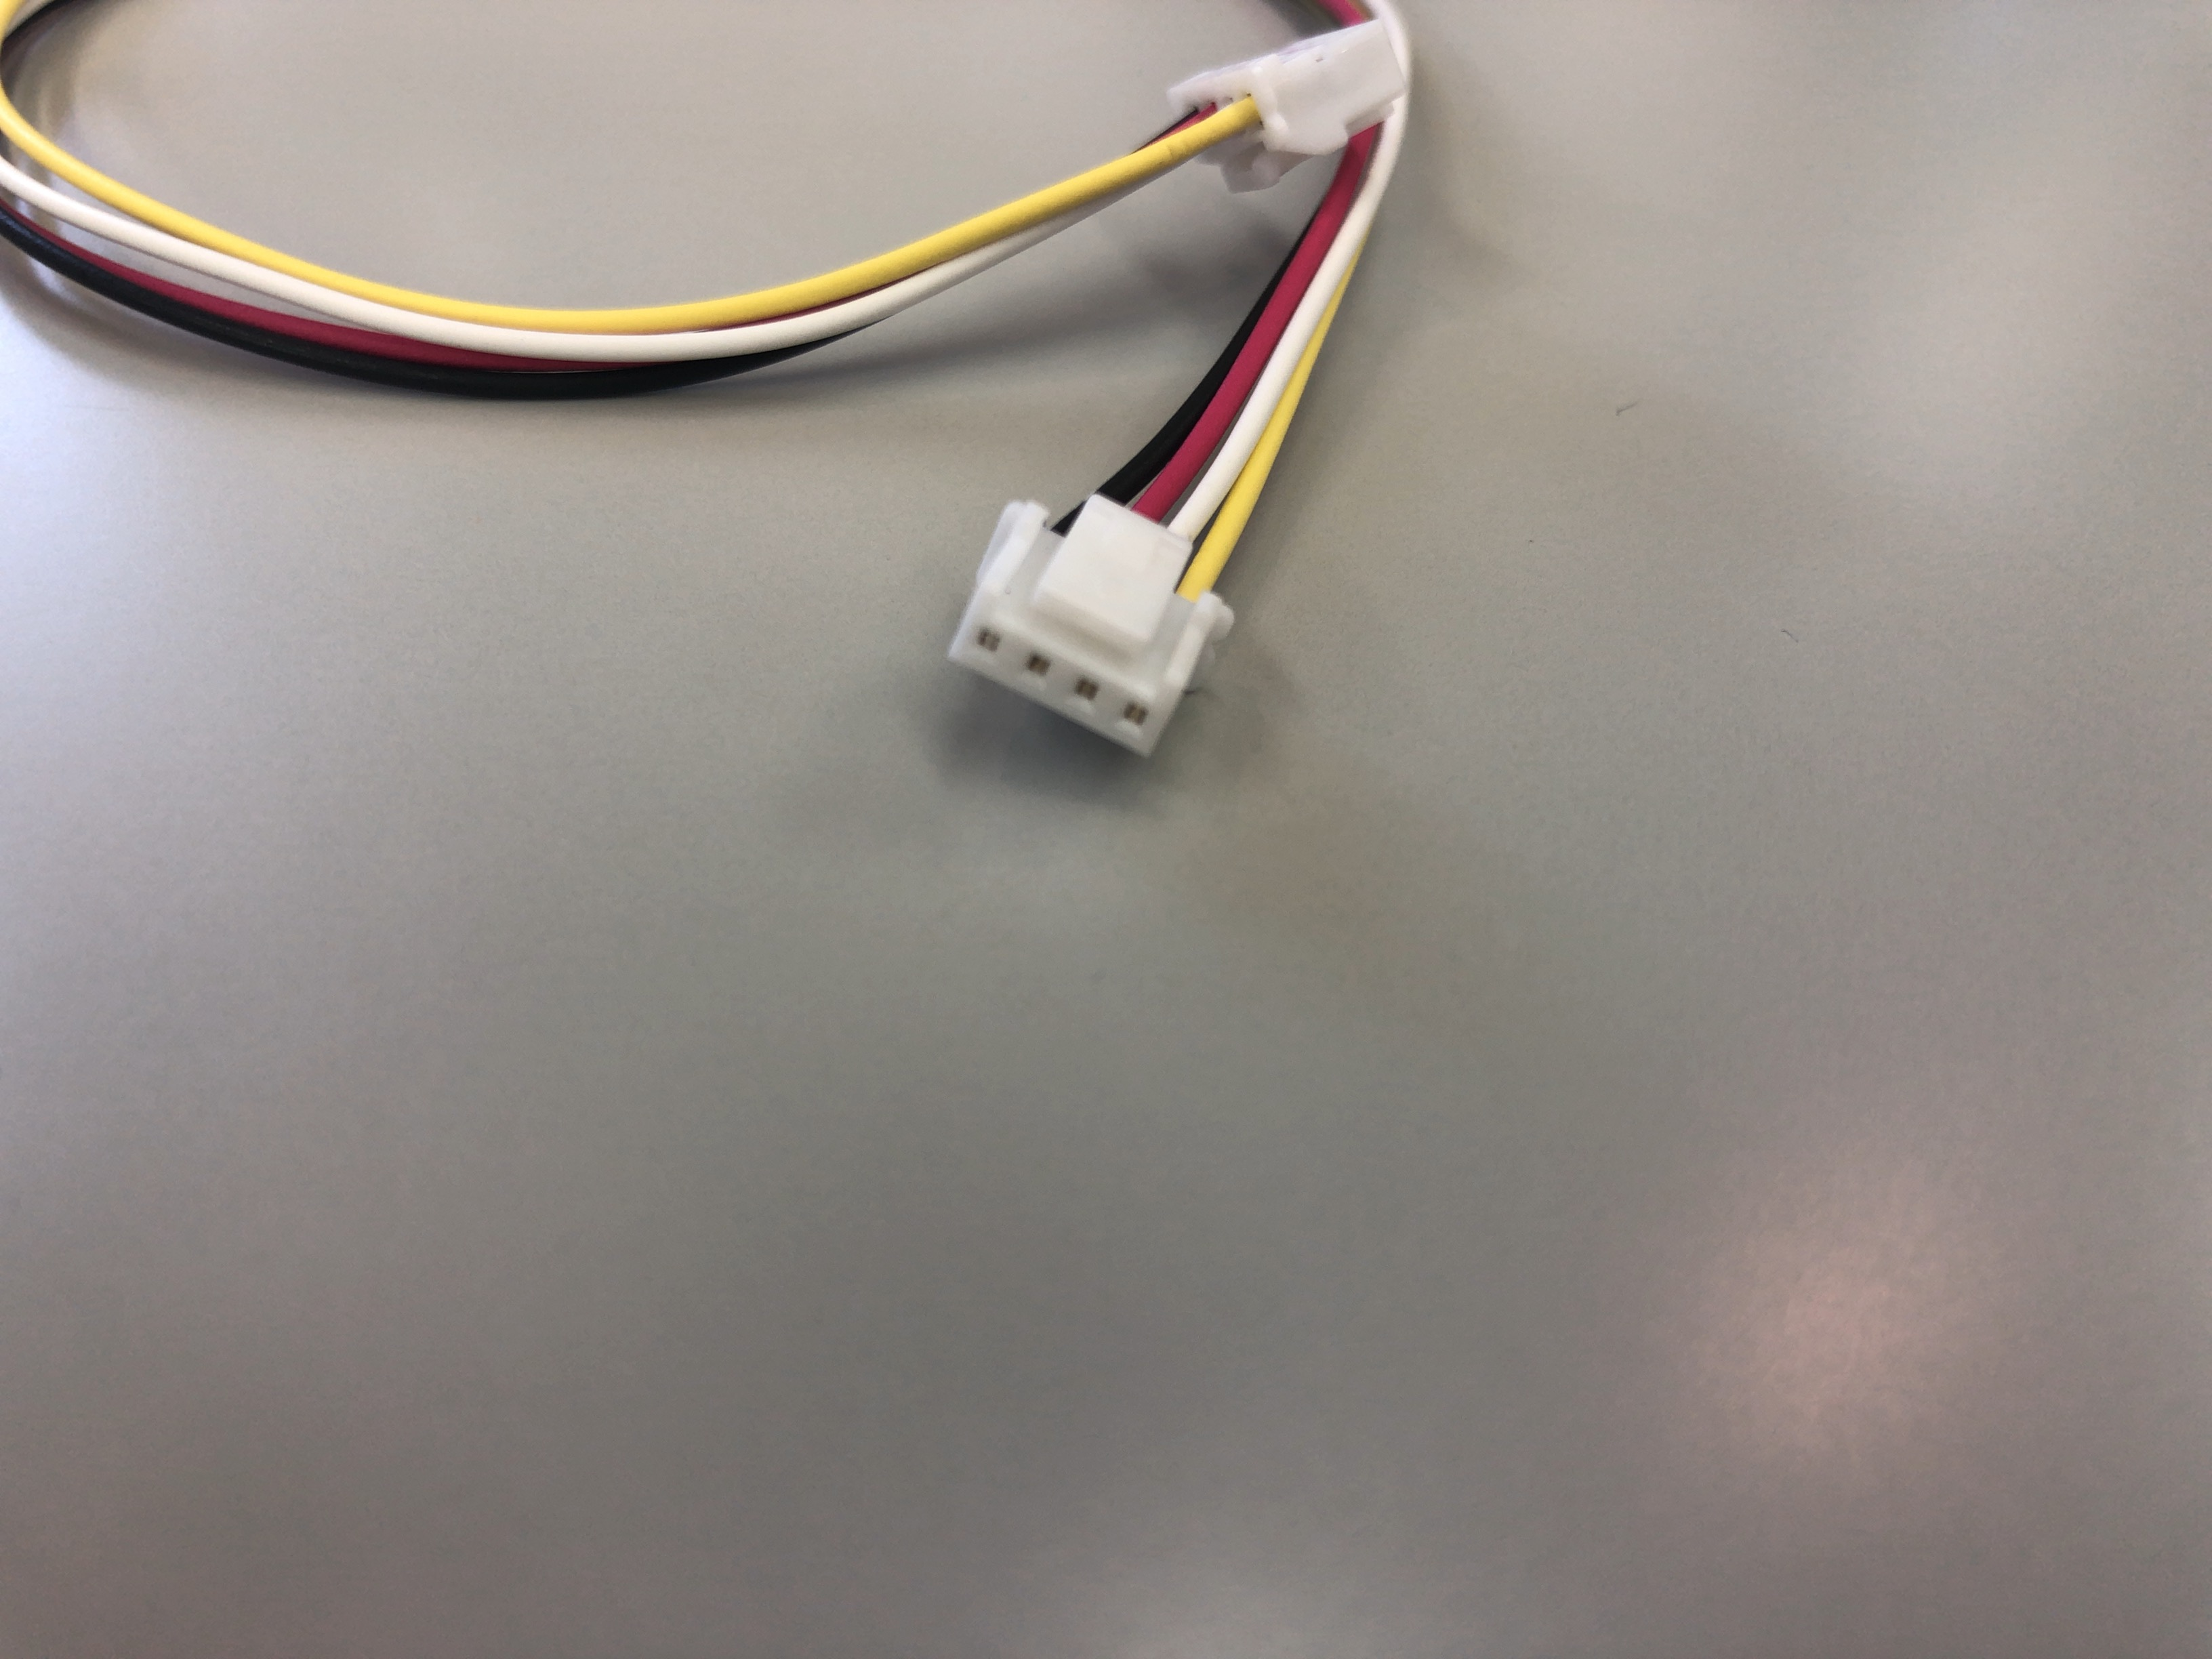
\includegraphics[width=0.8\hsize]{images/chap05/text05-img014.jpg}
    \caption{4ピンケーブル(コネクタ)}
  \end{minipage}
  \hspace{0.04\columnwidth} % ここで隙間作成
  \begin{minipage}[t]{0.48\columnwidth}
    \centering
    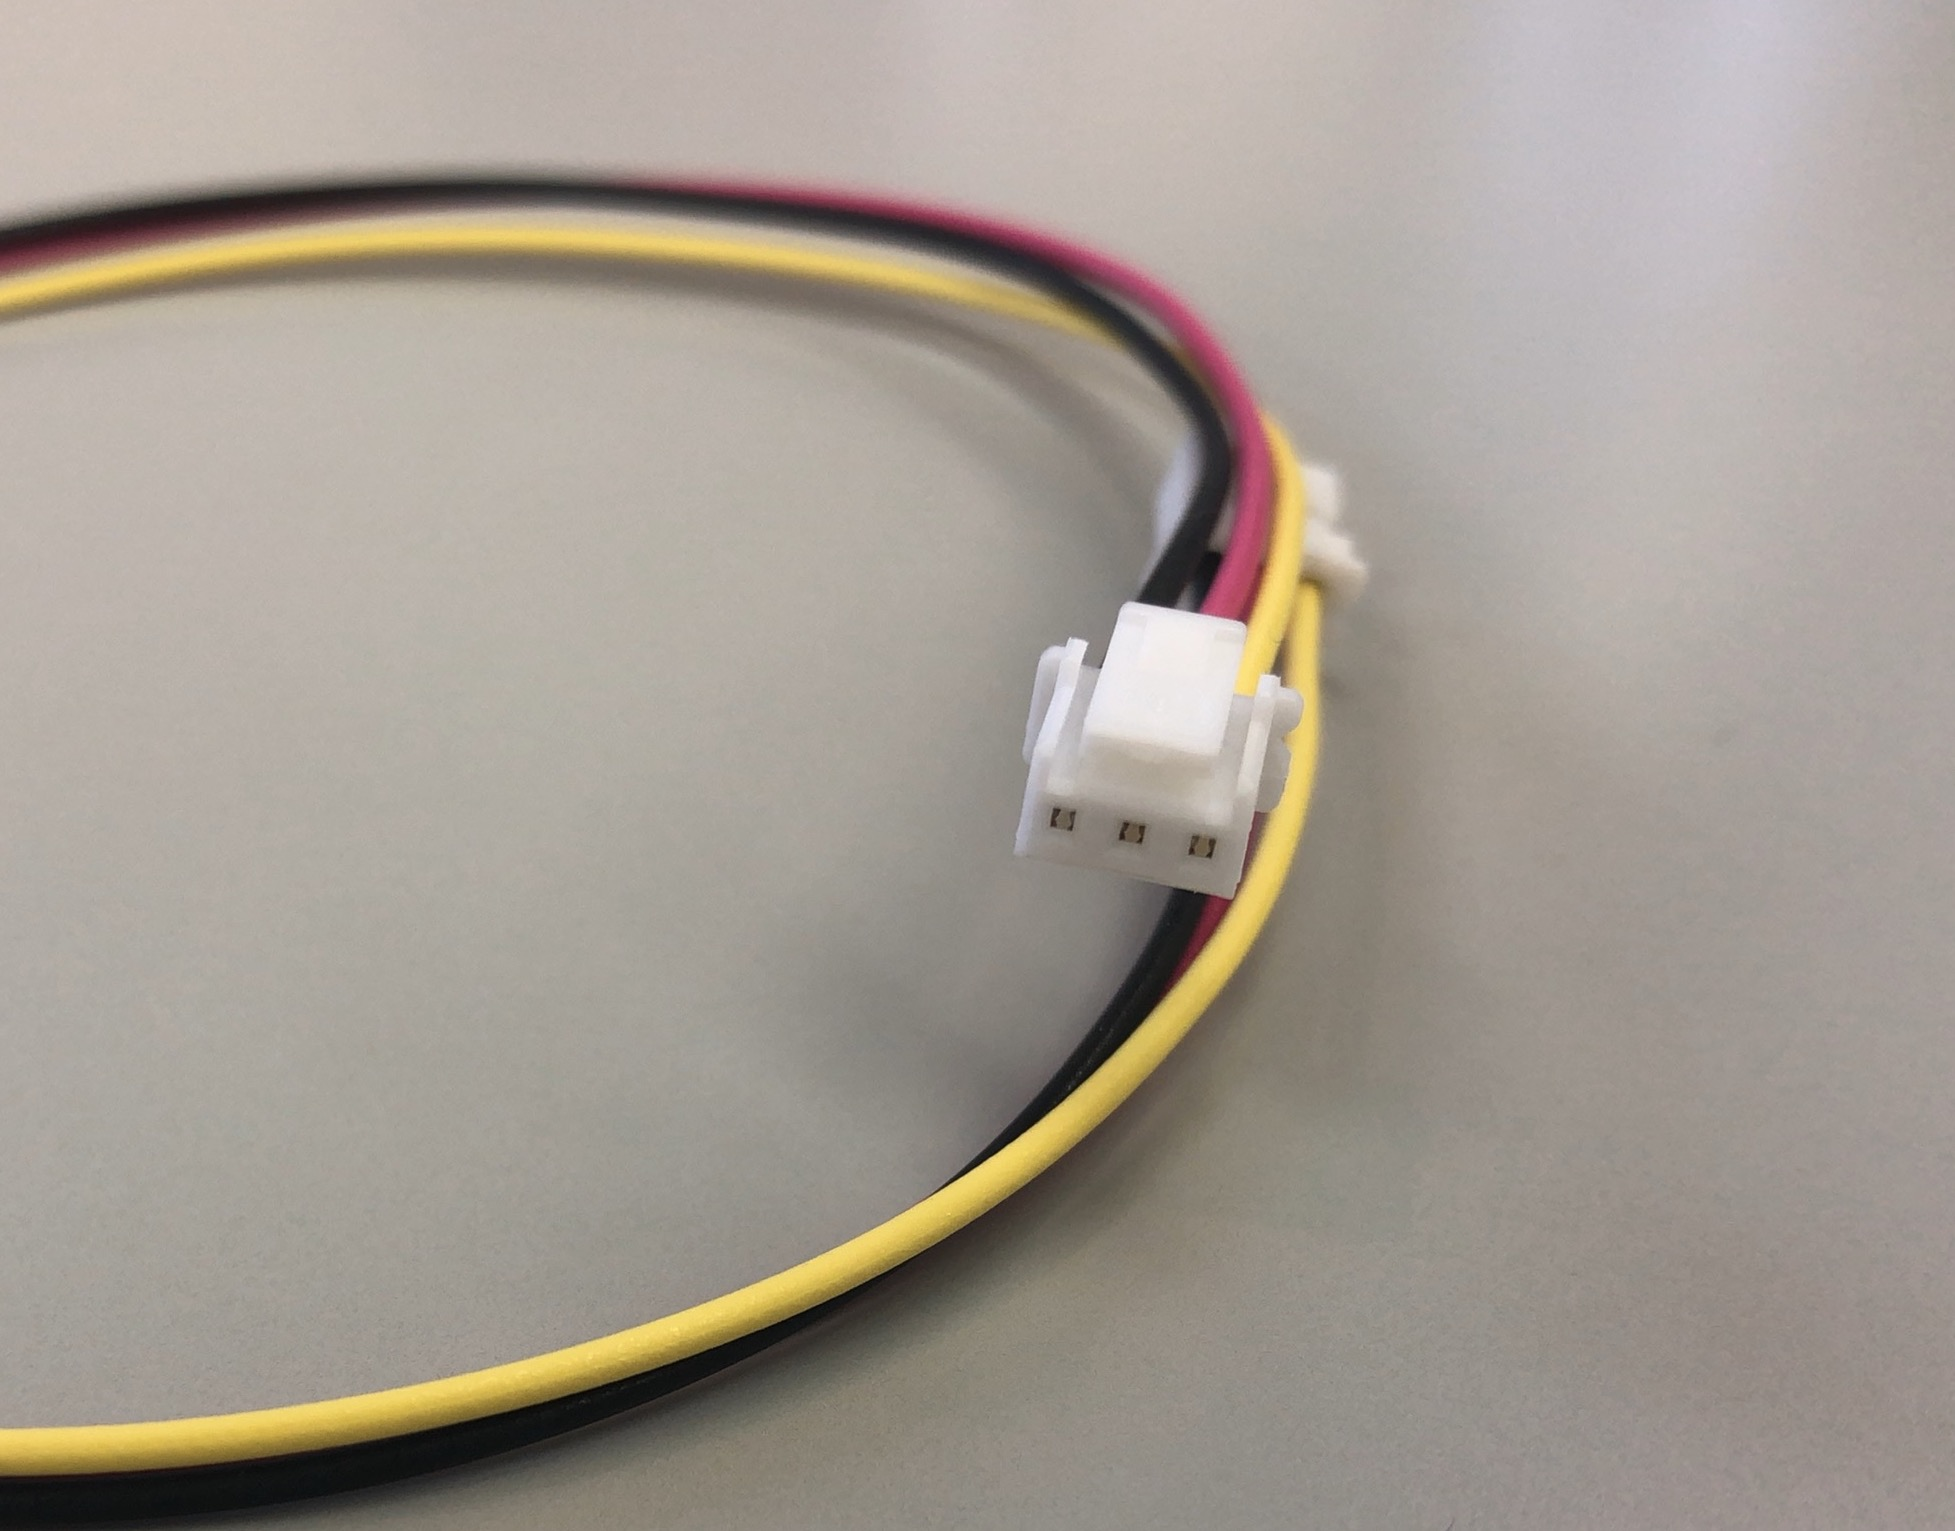
\includegraphics[width=0.8\hsize]{images/chap05/text05-img015.jpg}
    \caption{3ピンケーブル(コネクタ)}
  \end{minipage}
\end{figure}











